% !TEX root = ../Documentation.tex

\section{Design}
\label{sec:design}

\subsection{System overview}
  The parser module overview is given in \autoref{fig:ParserModules}.
  Each of the modules are described in the following subsection.
  %
  \begin{figure}[ht]%
    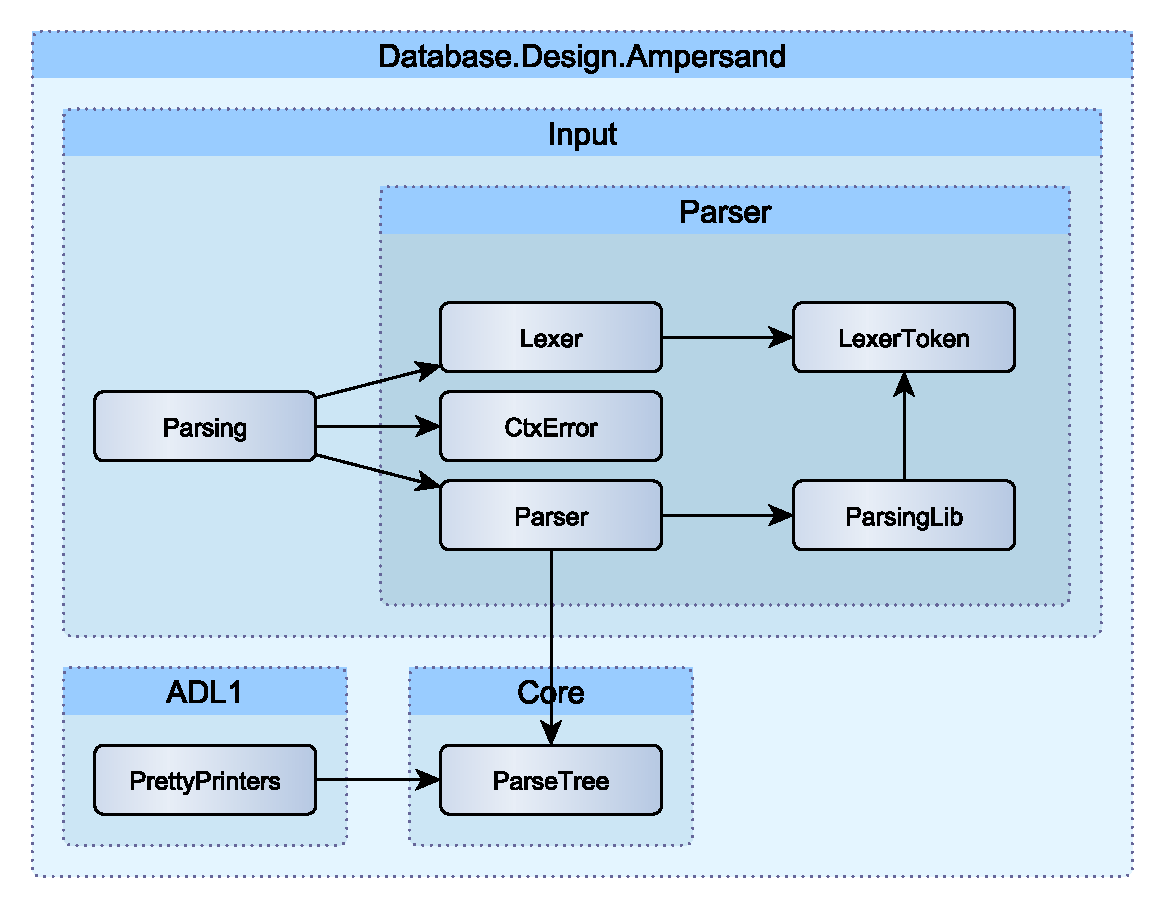
\includegraphics[width=\columnwidth]{Figures/ParserModules}
    \caption{The parser modules and their relationships}
    \label{fig:ParserModules}
  \end{figure}%

  \subsubsection{Modules}
  \label{subsec:parser-modules}
  In this section a short description of each module is given:%
  %
  \begin{description}
    \item[Parsing] module that implements the interface of the parser with the rest of the system.
      It is responsible for reading the input files, calling the lexer and the parser and returning a parse tree as result (or a parse error).

    \item[Parser] module responsible for executing the parsing itself.
      It accepts the tokens that are allowed in each grammar production and generates the corresponding parse tree.
      The parser is described in \autoref{subsec:parser}.
      
    \item[ParsingLib] library that contains several useful functions to assist the parser, e.g. token recognition.
      These functions are not depending on the specific grammar rules.
      
    \item[ParseTree] external module containing the parse tree data structures.
      Only details of this module have been changed during this project (e.g. field ordering).
    
    \item[PrettyPrinters] contains the \texttt{Pretty} class and the functions responsible for printing the parse tree to ADL scripts in a `pretty' way.
    
    \item[CtxError] contains the data structures responsible for the parse errors and their location.
      This module has not been refactored as a part of this project.
    
    \item[Lexer] module responsible for recognizing the input characters and converting them to tokens.
      The lexer is described in \autoref{subsec:lexer}.
    
    \item[LexerMonad] contains a monad definition that supports lexing with context.
      It tracks for example the location in the input and the warnings that may be generated.
    
    \item[LexerMessage] contains functions to handle errors and warnings from the lexer.
    
    \item[LexerBinaryTrees] module responsible for searching binary trees in an efficient way, to support the token recognition.
    
    \item[LexerToken] contains the data structure that represents the input tokens for the lexer.
      The tokens work as an interface between the lexer and the parsing library.
  \end{description}

\subsection{Changes due to Parsec}
TODO: Show the differences between uulib and Parsec, e.g. the try for backtracking.

\subsection{Lexer}
\label{subsec:lexer}
TODO: describe how the lexer works, and the improvements done to it.

\subsection{Parser}
\label{subsec:parser}
TODO: describe how the parser is implemented.

\subsubsection{Backtracking}
TODO: describe why the try-statements are necessary.

\subsection{Errors}
TODO: show what we've done to improve the errors.

\subsection{Next steps}
TODO: give tips on how to further improve the parser. e.g. cleanup CtxError, add warnings, use <?> for the errors...